\documentclass[12pt]{article}
\usepackage[utf8]{inputenc}
\usepackage[left=1.5in, right=1in, top=1in, bottom=1in, includefoot, headheight=13.6pt]{geometry}
\usepackage{biblatex}
\usepackage{graphicx}
\usepackage{amsmath}
\newtheorem{theorem}{Theorem}
\addbibresource{bib.bib}
\graphicspath{ {./figures/} }

\title{Network Complexity}
\author{Yipei Zhao}
\date{\today}

\begin{document}
\begin{titlepage}
    \begin{center}
        \vspace*{1cm}
            
        \Huge
        \textbf{Network Complexity}
            
        \vspace{0.5cm}
        \LARGE
        Thesis Subtitle
            
        \vspace{1.5cm}
            
        \textbf{Yipei Zhao}
            
        \vfill
            
        A dissertation presented for the degree of\\
        Master of Science
            
        \vspace{0.8cm}
            
        
\includegraphics[width=0.4\textwidth]{university.png}
            
        \Large
        MSc Data Analytics\\
        Aston University\\
        United Kingdom\\
        05 September 2021
            
    \end{center}
\end{titlepage}
\section{Introduction}
In my literature review, several complexity measures were introduced, includes the theory and the difference between them. 
\subsection{Random graphs}
We have many real networks in the actual world, but defining or observing every one of them is not feasible. For simulation and comparison reason, network scientists introduced the idea of random network. They are also known as Erdos-Renyi network in honour of two mathematicians: Pal Erdos and Alfred Renyi. They have important contributions to understand the properties of a random network\cite{barabási2016network}\\
\noindent
There are two definitions of a random graph:
\begin{itemize}
    \item $G(n,p)$ network. A graph with $n$ nodes will be initialised, there will be at most $(n)(n-1)/2$ edges. Every edge will have a probability $p$ to be instantiate. This approach brings a randomness propertyto the graph; number of edges $m$. A $G(n,p)$ graph returns a fixed $n$ but a different $m$ everytime. The expectation of $m$ is $p(n)(n-1)/2$., but usually comes with a small difference.
    \item $G(n,m)$ or $G(n,L)$ network. A graph with $n$ nodes will be initialised, $m/L$ edges will be connected from a random node to another random node. Due to the non-randomness of $G(n,m)$ networks, they are used to simulate the behaviour of a random network in this thesis.
\end{itemize}
\subsubsection{Random graphs parameter}
In the literature review, we introduced the idea of clustering coefficient and average distance. For a random graph, the clustering coefficient and average distance can be calculated using formulas.\cite{barabási2016network} The average clustering coefficient of a random graph is $p$, or $2m/((n)(n-1))$(number of instantiated links divided by total number of possible links). Clustering coefficient is used to illustrate the ratio between connected links and possible links. If there are $k$ neighbours of a node, there can be at most $k(k-1)/2$ between the neighbours. In these $k(k-1)/2$ links, only $p$ of them will be instantiated. Thus, the ratio of connected links and possible links becomes $\frac{pk(k-1)/2}{k(k-1)/2}=p$. Additionally, average distance of a random graph is $\langle d\rangle \approx \frac{ln(n)}{ln\bar (k)}\approx \frac{ln(n)}{ln(2m/n)}$. To be noticed, both parameters are expectation/approximated, they won't be exact for a random graph.

\subsection{Small world}
About 50 years ago, a famous study was carried out by Standley Milgram\cite{milgram1967small} in the interest of this question: how many intermediates are needed to pass a message between two irrelevant person? This is known as the small-world problem. As counterintuitive as it may seem, the medium number of intermediates needed is only 5(an average of 6). This is not a non-bias experiment and it is almost impossible to determine the actual number of intermediates needed in mordern world. Nevertheless, this number would be smaller than most peoples' expectation. Mathematically, the small world problem is the study of graphs with small path length. Previously, we introduced the formula to calculate the average distance $d_r$ of a random graph. Thus, if a graph has $d/d_r <1$, this graph has less average distance than random graphs. If the ratio $d/d_r$ is relatively small, we can classify it as a small-world network.\\

\subsubsection{Watt-Strogatz graph and Newman-Watts graph}
A small-world network can be generated by Watt-Strogatz model\cite{wsmodel} and Newman-Watts model.


\section{Methods}
\subsection{Implemeted methods}
In the literature review, 9 methods were introduced, 7 methods were succesfully implemented and tested with a new method $MAri$ based on the idea of $MAg$. The implemented methods are:
\begin{itemize}
    \item Subgraph measures:
    \begin{itemize}
        \item $C_{1e,st}$
        \item $C_{1e,spec}$
        \item $C_{2e,spec}$
    \end{itemize}
    \item $OdC$ (Entropy measure)
    \item Product measures:
    \begin{itemize}
        \item $MAg$
        \item $Cr$
        \item $Ce$
        \item $MAri$
    \end{itemize}
\end{itemize}

\subsection{$MA_{RI}$}
The $MAg$ measure is a product measure, which distributes higher complexity to graphs with medium number of edges and lower complexity at both tails. Using the product of redundancy $R$ and mutual information $I$, with a normalisation formular, $MAg$ is defined as\cite{KIM20082637}:
\begin{equation}
    \label{eq:MAg}
    \begin{gathered}
        R = \frac{1}{m}\sum_{i,j>i}ln(d_id_j)\\
        I = \frac{1}{m}\sum_{i,j>i}ln(\frac{2m}{d_id_j})\\
        MA_R = 4(\frac{R-R_{path}}{R_{clique}-R_{path}})(1-\frac{R-R_{path}}{R_{clique}-R_{path}})\\
        MA_I = 4(\frac{I-I_{clique}}{I_{path}-I_{clique}})(1-\frac{I-I_{clique}}{I_{path}-I_{clique}})\\
        MA_g = MA_R * MA_I
    \end{gathered}
\end{equation}
$R_{path},R_{clique},I_{path}$ and $I_{clique}$ represent lowest redundacy, highest redundancy, highest mutual information and lowest mutual information of graphs with fixed $m$ and $n$ respectively. The equations can be found in the literature review.\\
Even though $MA_g$ is well defined and normalised, a problem with the $MA_g$ is it does not assign highest complexities to graphs with the most middle number of edges for small graphs. The highest complexity is reached at $n^{1.5}$, instead of $\frac{n(n-1)}{4}$.\\

\begin{figure}[ht]
    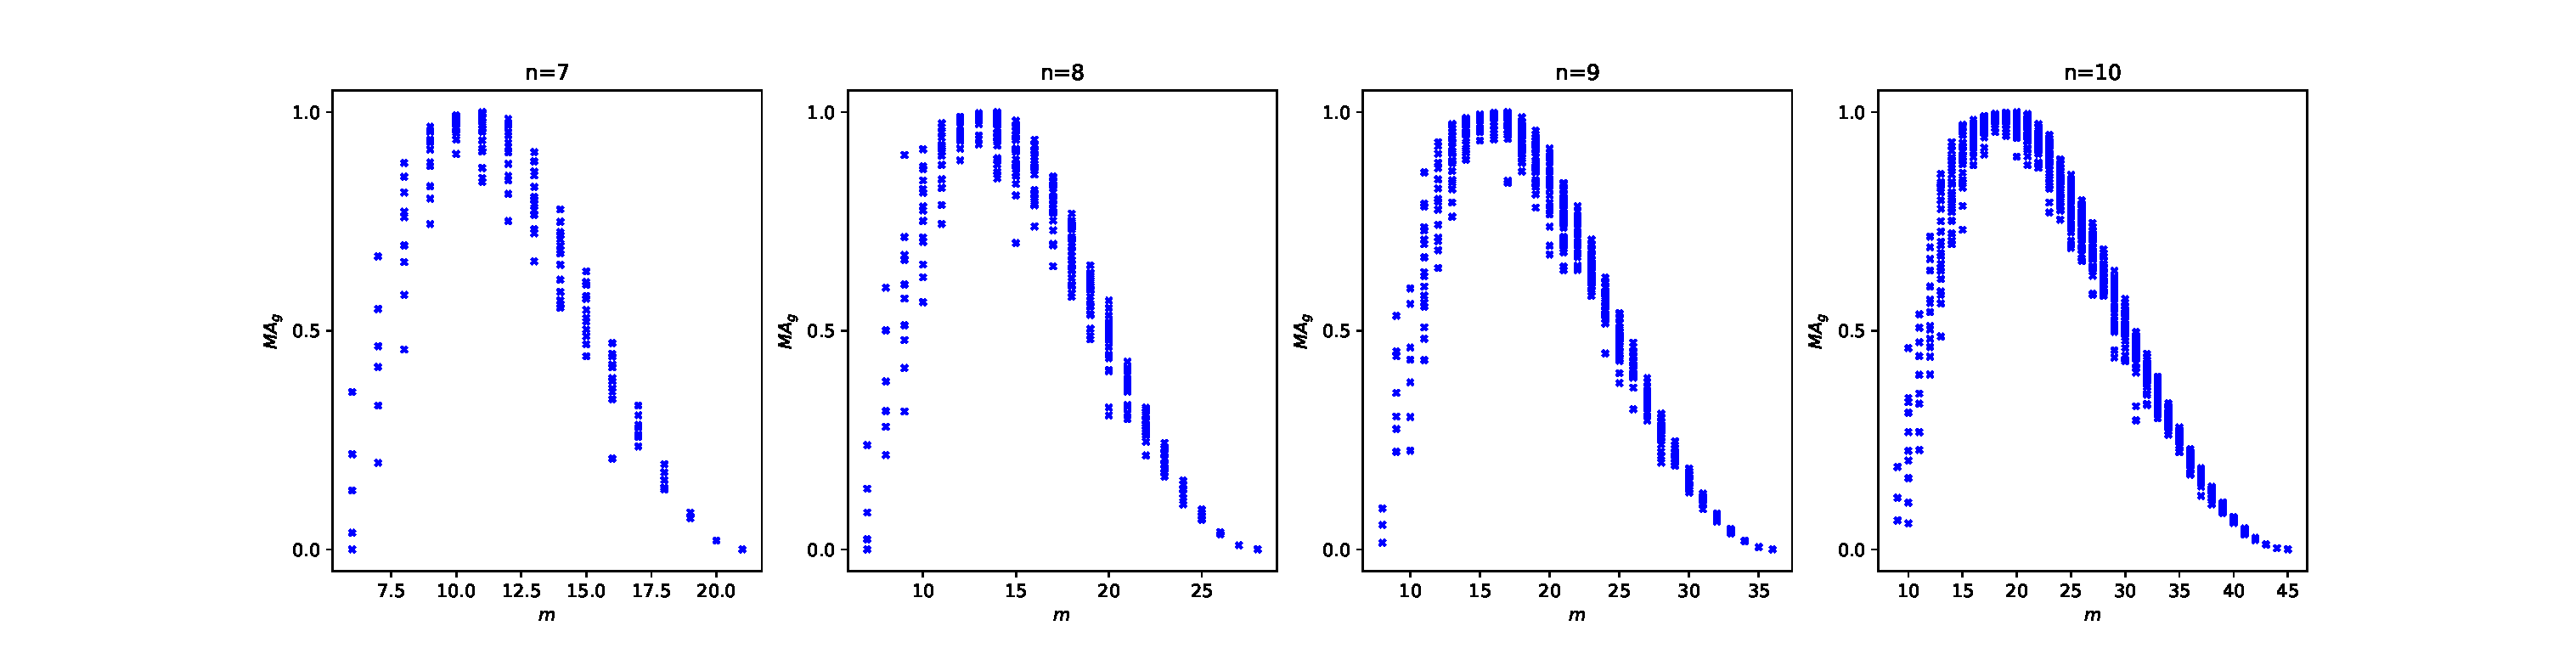
\includegraphics[width=\textwidth]{mag.eps}
    \centering
    \caption{$MA_g$ complexity values of graphs with n=7,8,9,10 nodes}
    \label{fig:mag}
\end{figure}
\noindent
Hence, we may change the normalisation term such that the highest complexity is shifted more towards the middle number of edges. The normalisation term becomes:
\begin{equation}
    \label{eq:mari}
    MA_{RI} = 4(\frac{R-R_{path}}{R_{clique}-R_{path}})(\frac{I-I_{clique}}{I_{path}-I_{clique}})
\end{equation}

\begin{figure}[ht]
    \centering
    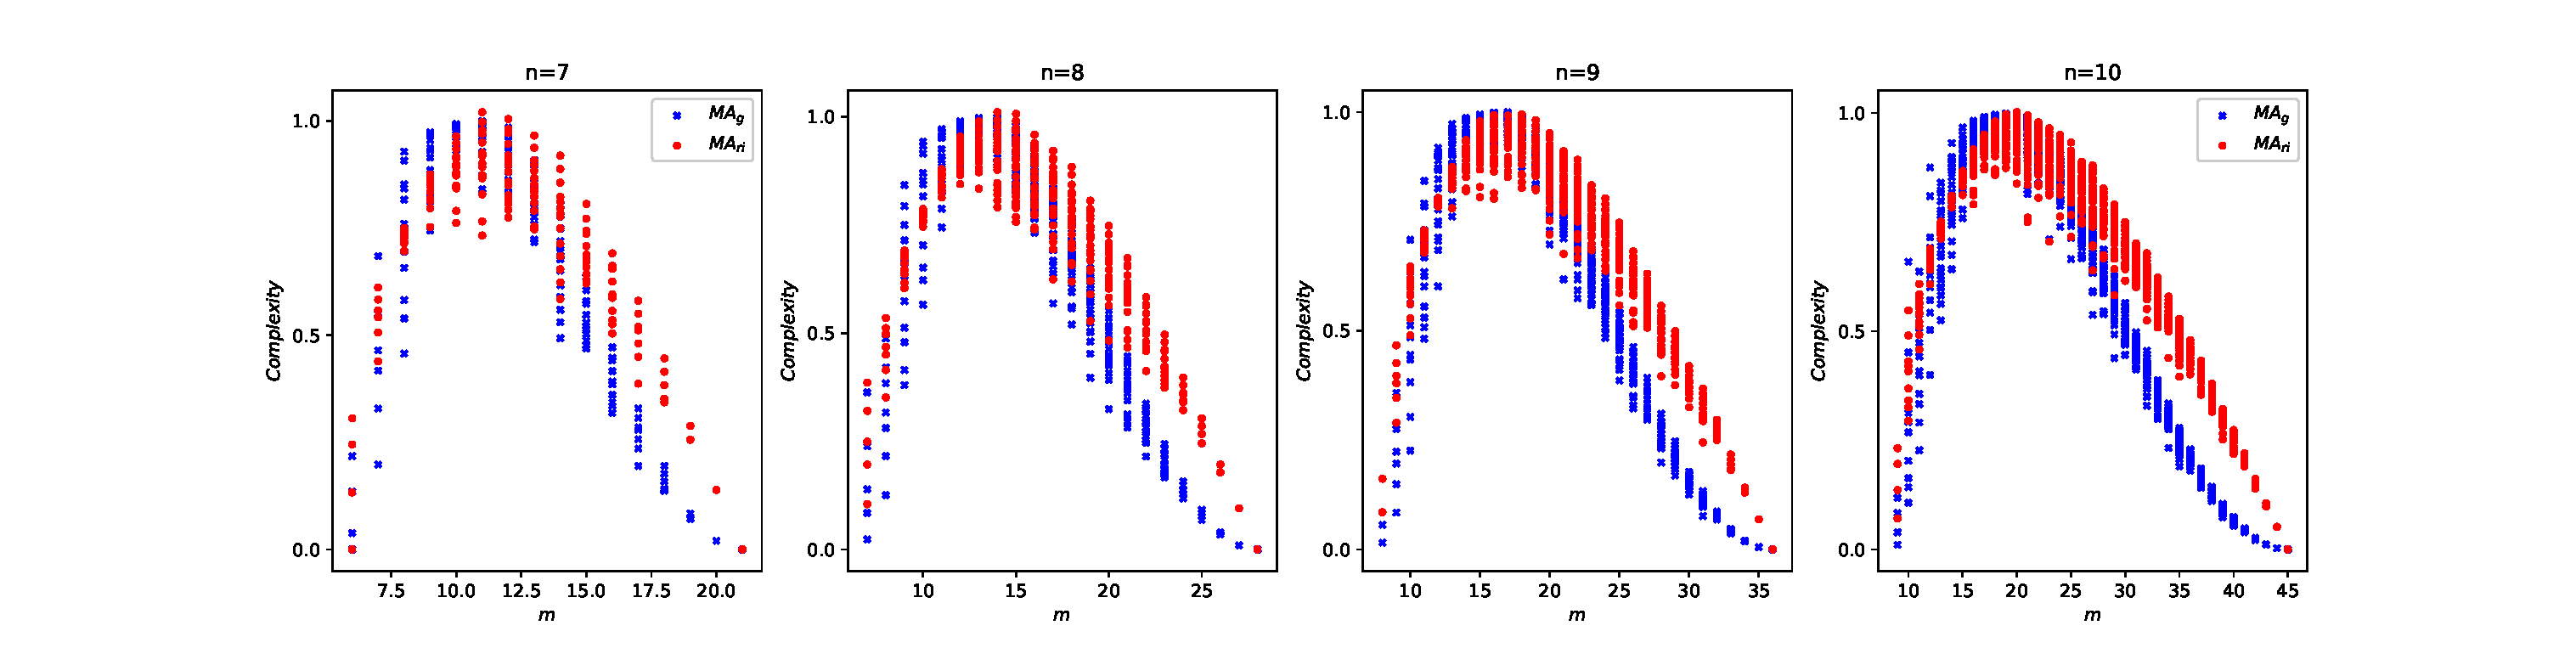
\includegraphics[width=\textwidth]{mag&mari.eps}
    \caption{Comparison of $MA_{RI}$ and $MA_{g}$.}
    \label{fig:mari&mag}
\end{figure}
\noindent
As showin in figure \ref{fig:mari&mag}, $MA_{RI}$ and $MA_{g}$ behave alsmost the same, whereas $MA_{RI}$ assigns higher complexity values to graphs with middle number of edges and averagely higher complexity than $MA_{g}$ for higher number of edges. The complexity of computation stays the same, which is $O(m)$. $MA_{RI}$ complexity intends to have the nomalization property, which is $0\leq MA_{RI}\leq 1$, with exceptions.\\
During the simulation, a few unnormalization cases were found, they are:\\
\begin{table}[h]
    \centering
    \begin{tabular}{|c|c|c|}
        \hline
        n & m & Highest complexity\\
        \hline
        6 & 9 & 1.0421694413111797\\
        \hline
        7 & 11 & 1.0203660524038531\\
        \hline
        7 & 12 & 1.0042984248515054\\
        \hline
        8 & 15 & 1.0068924792733018\\
        \hline
    \end{tabular}
\end{table}
\begin{figure}[ht]
    \centering
    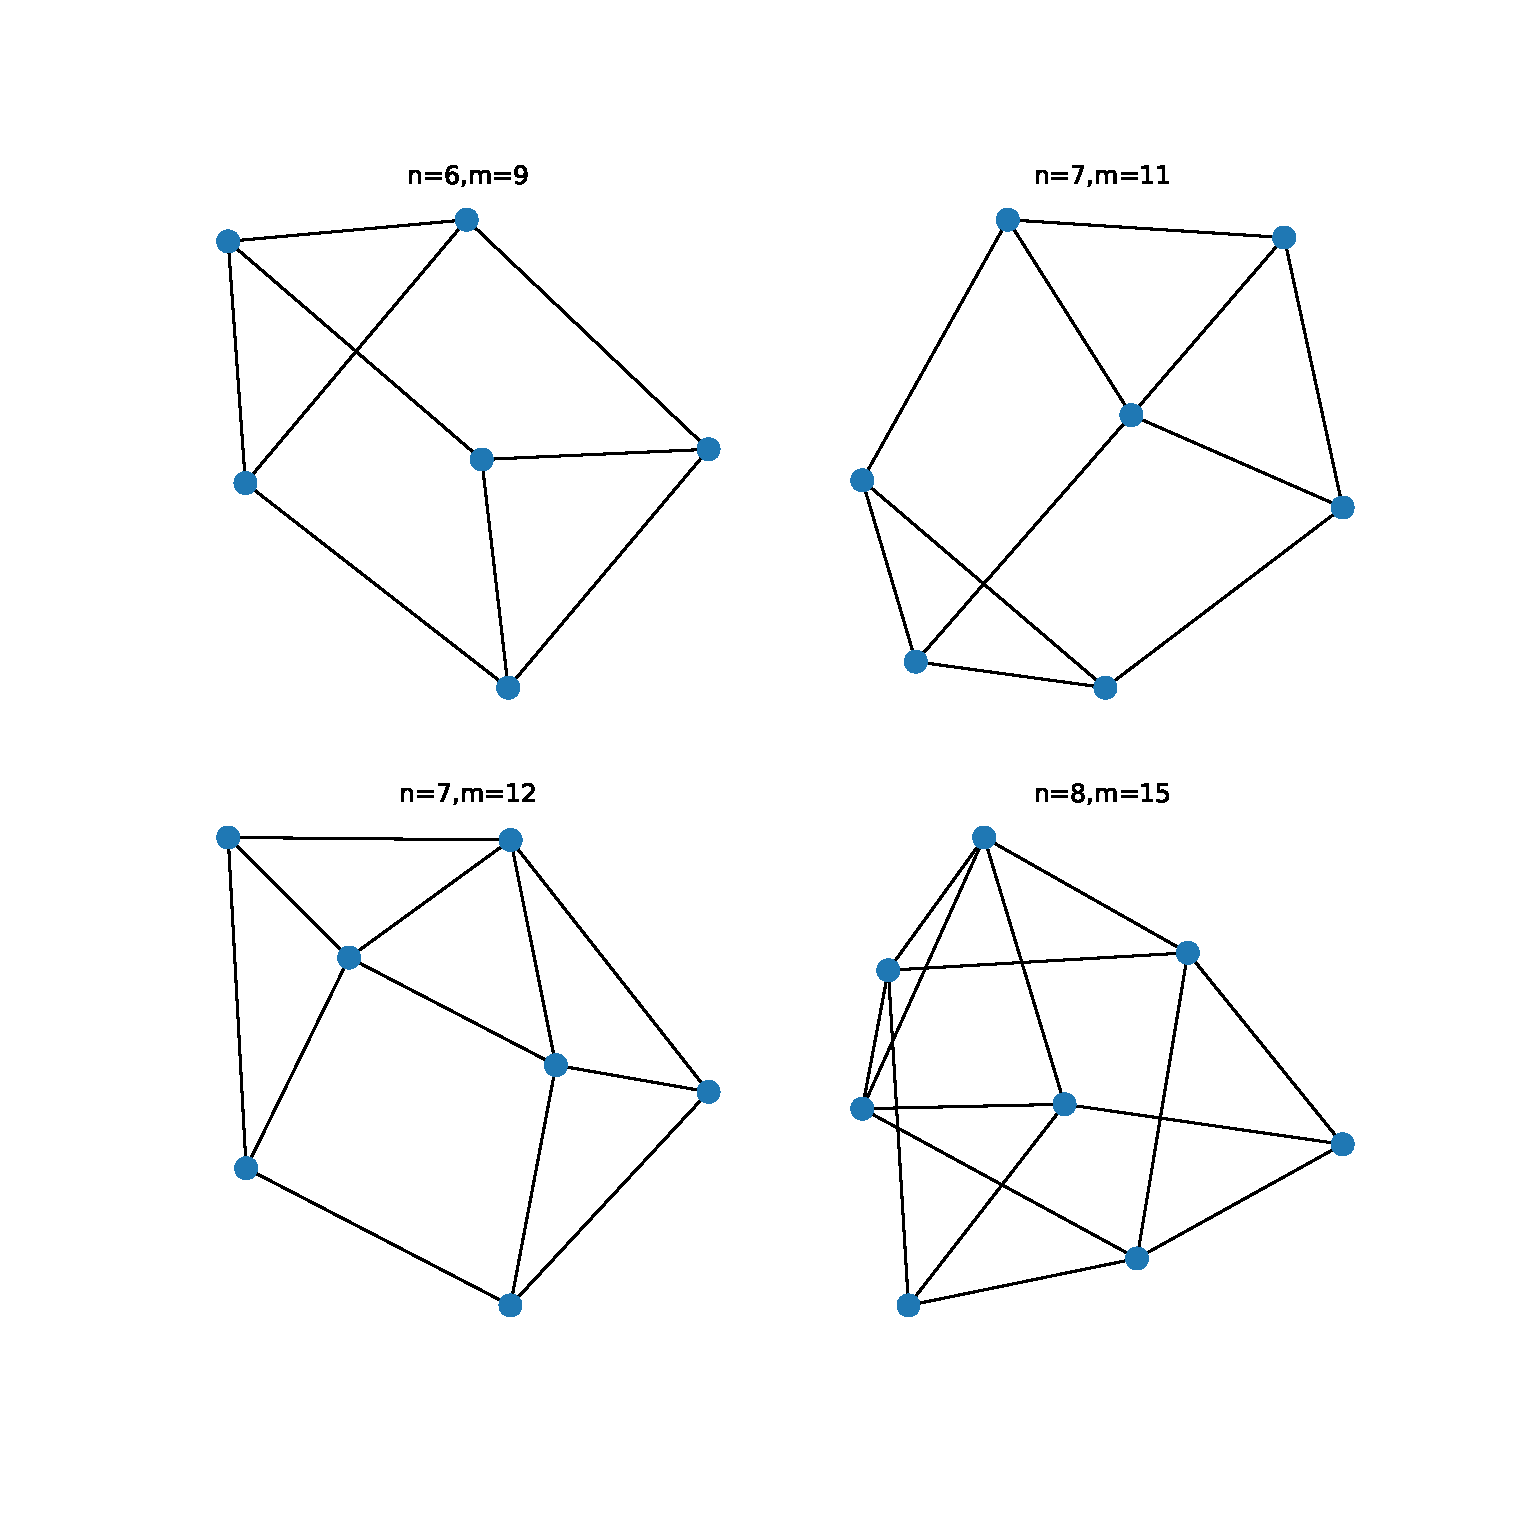
\includegraphics[width=0.7\textwidth]{mari_exception.eps}
    \caption{Graphs with highest $MA_{RI}$ complexity.}
    \label{fig:mari_execption}
\end{figure}
\noindent
These exceptions are only found for small graphs, for larger graphs, complexities are normalised. Therefore, a solution is proposed.\\
Observing the equation \ref{eq:mari}, the extremes are fixed for $n$, $R$ and $I$ are the variables. Also, $R$ and $I$ are negatively correlated with correlation coefficent equal to -1.\\
\begin{equation}
    \label{eq:ricorrelation}
    \begin{gathered}
        R = \frac{1}{m}\sum_{i,j>i}ln(d_id_j)\\
        I = \frac{1}{m}\sum_{i,j>i}ln(\frac{2m}{d_id_j})\\
        I = \frac{1}{m}\sum_{i,j>i}ln(2m)-\frac{1}{m}\sum_{i,j>i}ln(d_id_j)\\
        I = ln(2m)-R\\
    \end{gathered}
\end{equation}
Thus, if the maximum of $\sum_{i,j>i}ln(d_id_j)$ can be found, the maxmimum of $MAri$ can be found as well. The maximum can be found in two ways:\\
\begin{itemize}
    \item Creates all graphs with the respective $n$, and find the maximum complexity, and divide all valeus by the maximum complexity.
    \item As $R$ and $I$ are negatively correlated with coefficent -1, we can find the maximum of $MAri$. Given the fact $R_{min} = R_{path} = ln(2m)-I_{max} = ln(2m)-I_{path}$ and $R_{max} = R_{clique} = ln(2m)-I_{min} = ln(2m)-I_{clique}$. By varying the value of $R$ between $R_{min}$ and $R_{max}$, $MA_{RImax}$ can be found.
\end{itemize}
We only suggest to use the solutions for small graphs, not only the problem only occurs for small graphs, but also the complexity will be largely increased for large graphs.\\
\subsection{Potential problems and solutions of different subgraph measures}
During the implementation of measures, several problems were found, possible solutions are also given for future projects.\\
Different subgraph measures are principally simple, but they are complex to compute, within at least $O(n^2)$ time\cite{KIM20082637}. This is not the only problem. An upper-bound of the complexity $m_{cu} = n^{1.68}-10$ was introduced by Kim and Wilhelm\cite{KIM20082637} to normalise the complexity. However, from the simulation, we found that this may not be the actual upper-bound of the different subgraph measures.

\begin{figure}[ht]
    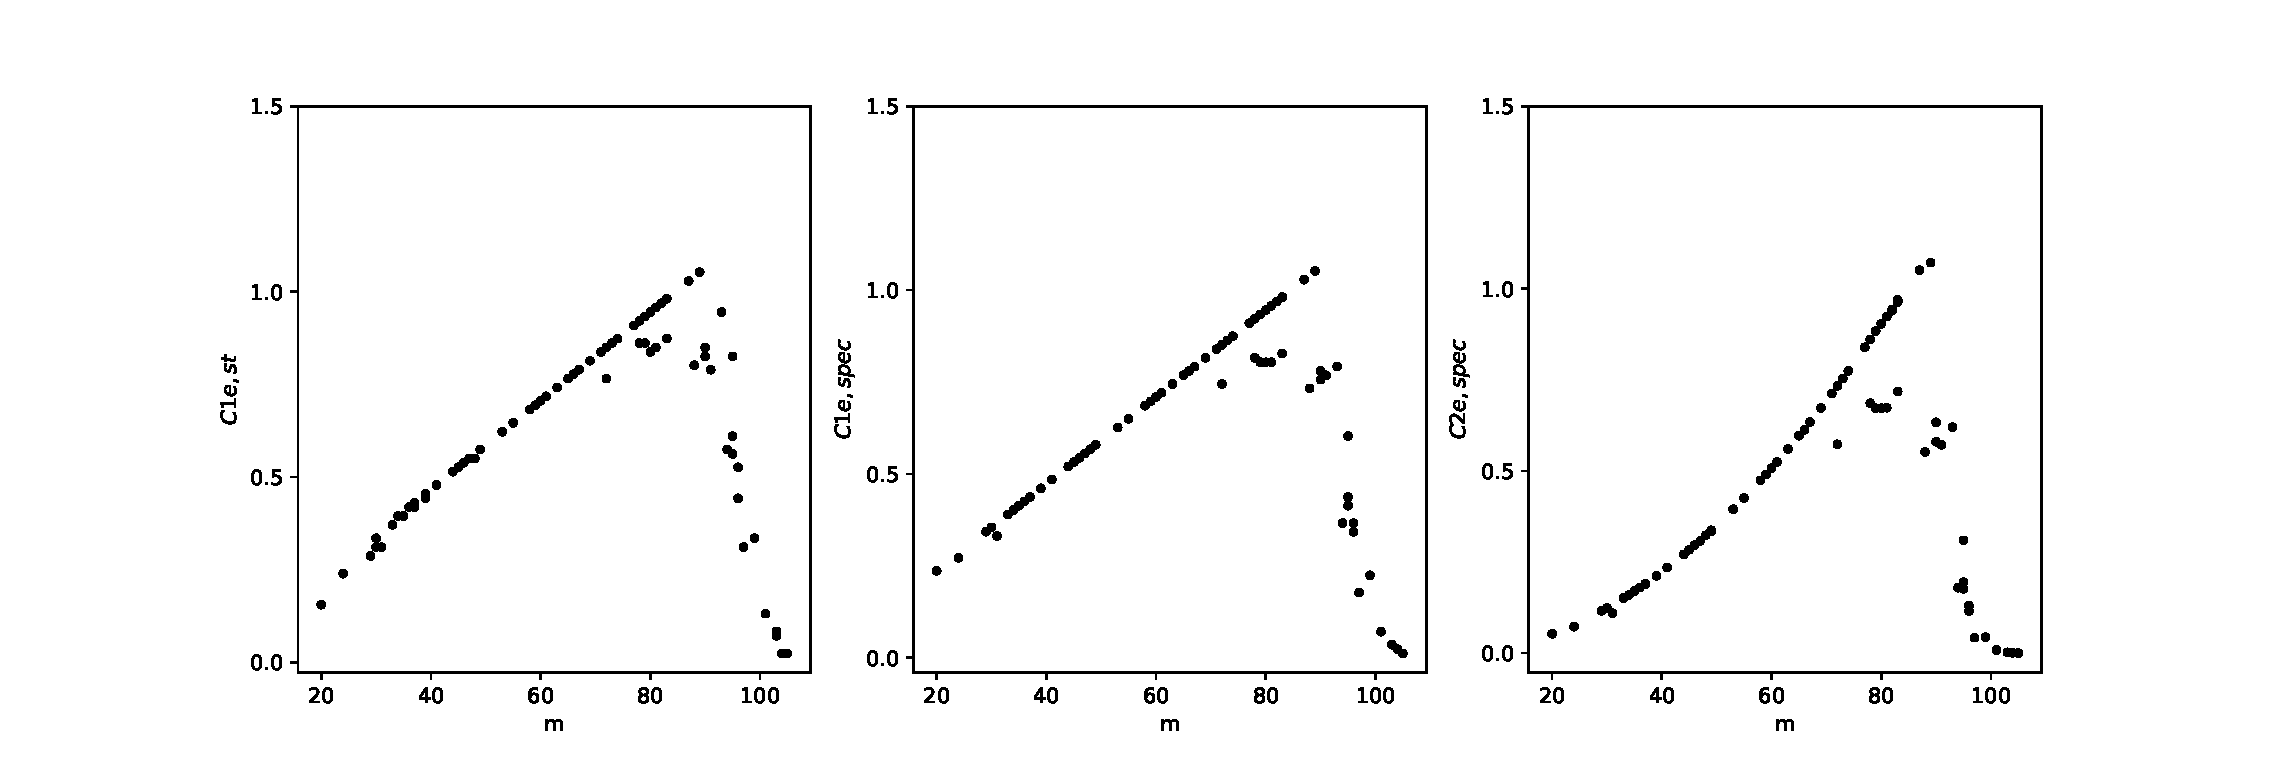
\includegraphics[width=\textwidth]{subgraph_measures.eps}
    \caption{Different subgraph measure of $G(n,m)$ random graphs, with $n$ = 15.}
    \label{fig:subgraph_measure}
\end{figure}
\noindent
The complexity is abnormal for graphs with around 90 edges and 15 nodes as shown in figure \ref{fig:subgraph_measure}. This could imply that the upper-bound $mcu$ is not correct, but there is another possible reason, which is the problem of floating point arithmetic.\\
On most machines today, numbers are represented in binary system\cite{floating_point}. For example, 0.2 is 0.00110011001100110011... in a binary system. This series is infinite, represented by $1*2^{-3}+1*2^{-4}+1*2^{-7}+1*2{-8}...$. For obvious reasons, computer scientists don't want to work with infinite series, therefore, the series is approximated. On a modern compueter, the series is usually approximated to 63 digits with 1 digit represents the sign of the number. After approximation, the error could cause the equal operation to fail. A well known example is that for modern programming language or machine that operates this numbering system, 0.2+0.1 does not equal to 0.15+0.15. As a result, the comparison may cause more number of different subgraph than actual.\\
The core of different subgraph measure is to compare the cofactor($C_{1e,st}$)/spectrum($C_{1e,spec}$ and $C_{2e,spec}$) of a subgraph. Given the fact that the proabbility of a decimal number to appear in the sprectrums is high and the cofactor will also be very large for a large graph. The comparison will be inaccurate. There are three possible solutions:
\begin{itemize}
    \item As suggested, errors will be made when approxiamted by the machine. An error threshold can be used when comparing spectrums and cofactors. For example, two numbers with relative error less than 1\% can also be considered as equal numbers. One disadvantage is the increase of complexity, taking more time and effort to compare the spectrums/number of spanning trees.
    \item Similarly, numbers can be rounded before comparison to avoid error. This is used in the implementation of different subgraph measures, all cofactors and spectrums are rounded to first 10 significant figures. This solution requires less computation time than first solution. The drawback is that similar graphs can be considered as isomorphic graphs, this also applies to the first provided solution, but with higher accuracy for large graphs.
    \item Instead of using $m_{cu}$ as a normalisation parameter, $m$ can be used for one-edge-deleted subgraph complexity and $\genfrac(){0pt}{2}{m}{2}$ for two-edges-deletied subgraph complexity. This gurantees the normalisation and avoid the mistake that caused by the first two solutions, but on the other hand, causing the complexity to be different.
\end{itemize}
A unique problem with $C_{2e,spec}$ is the value is not properly normalised for small graphs.

\begin{figure}[ht]
    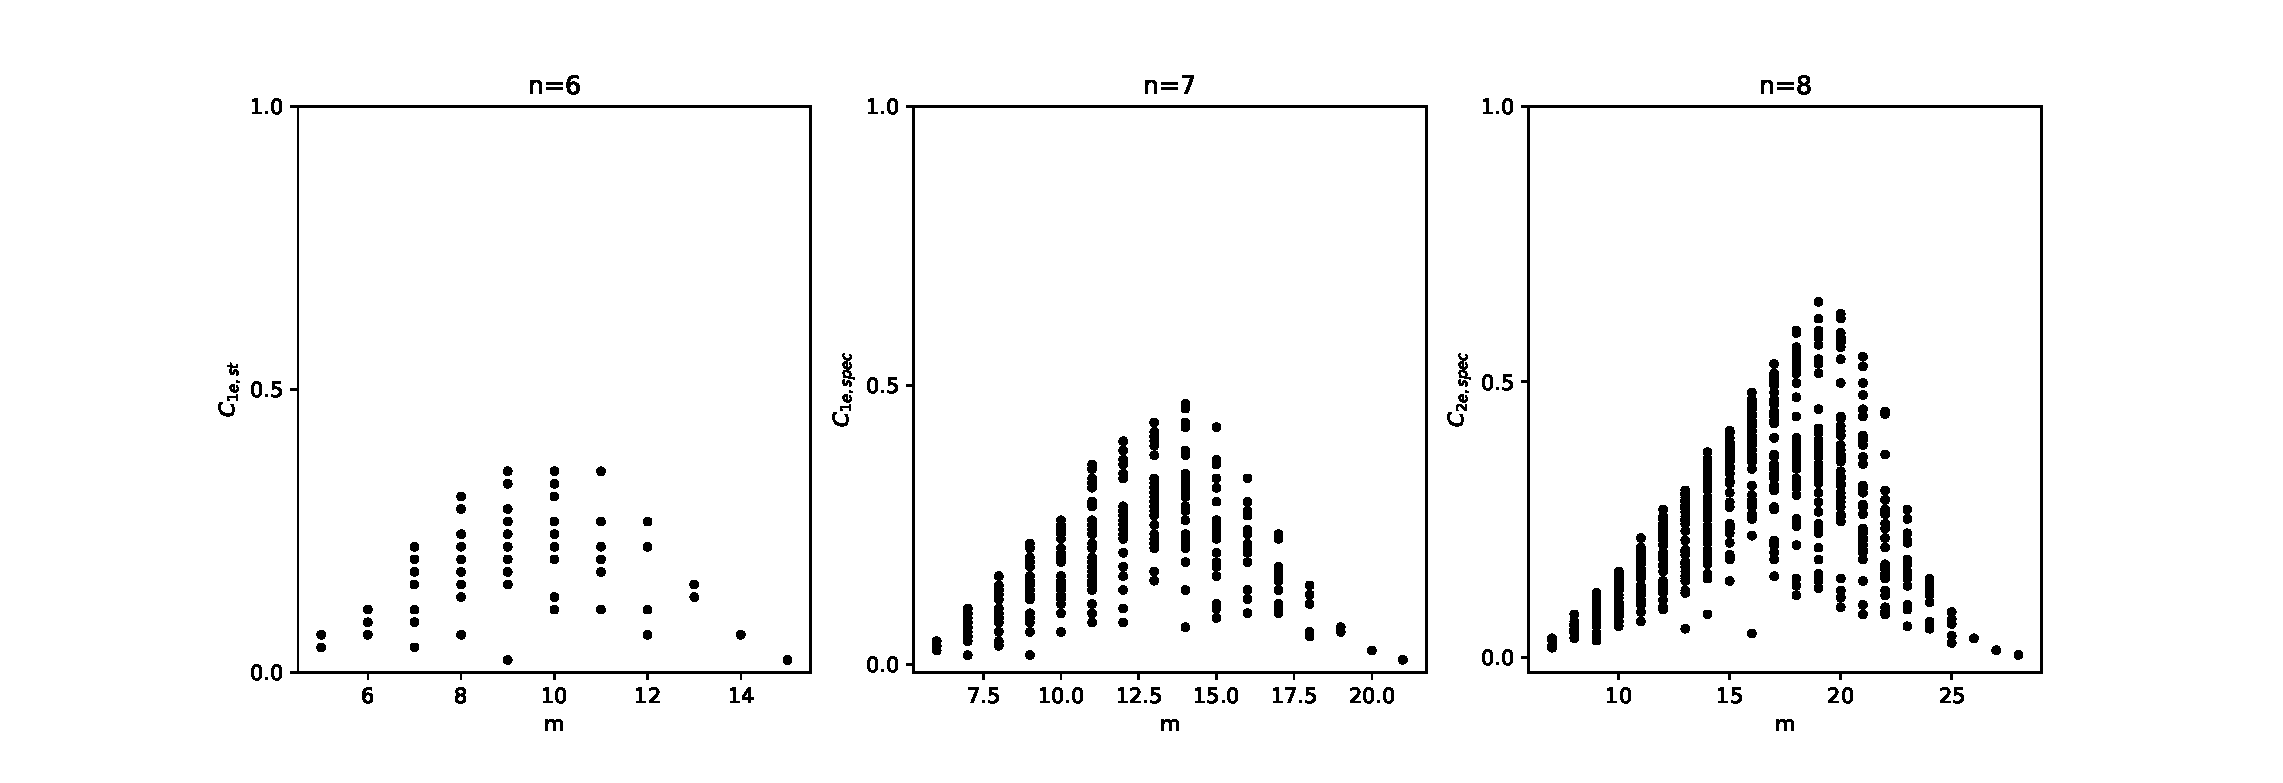
\includegraphics[width = \textwidth]{c2espec.eps}
    \caption{$C_{2e,spec}$ complexities for n = 6,7,8 respectively.}
    \centering
\end{figure}
\noindent
The upper-bound of $C_{2e,spec}$ is 0.5 while $ n\leq7 $. To have an upper-bound at 1, the complexity value have to be scaled by 2. However, scale by 2 will cause the complexity to exceed 1 for larger graphs. Thus, we sticked to the original normalisation and $C_{2e,spec}$ will have an upperbound at 0.5 for $n \leq 7$.

\section{Result}


\clearpage
\begin{figure}[ht]
    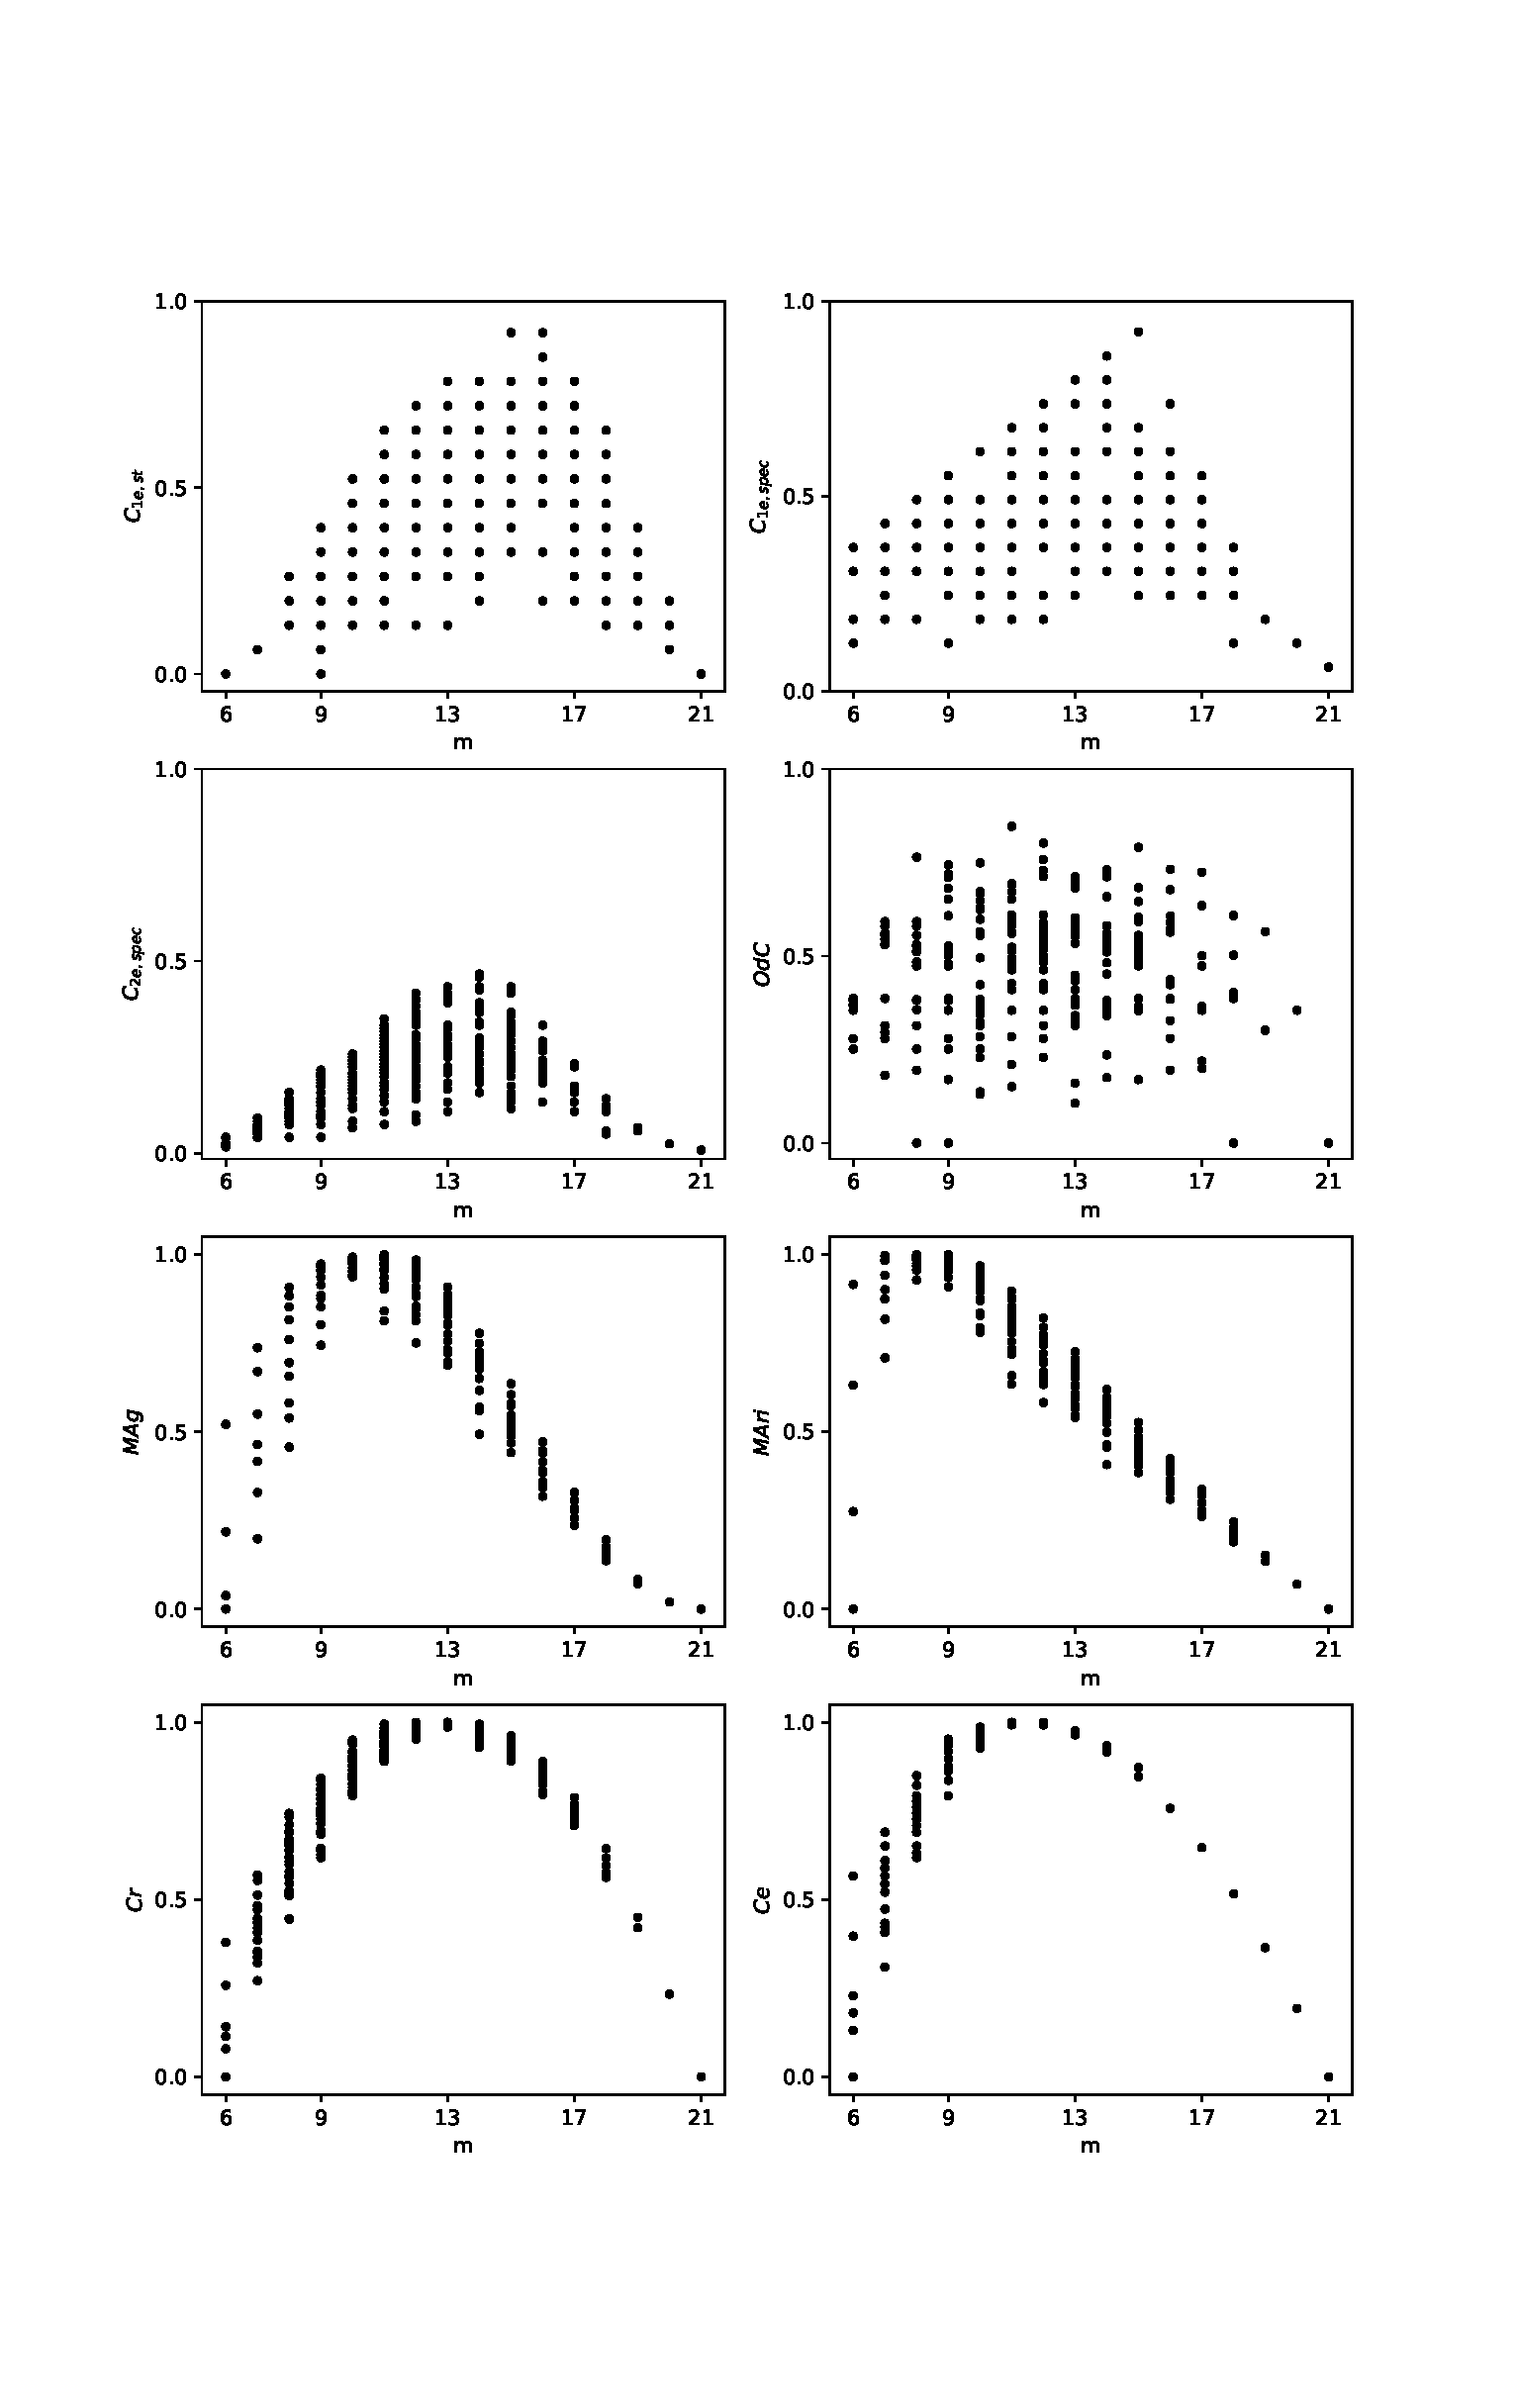
\includegraphics[width=\textwidth]{complexities.eps}
    \centering
    \caption{results of implemented methods of graphs with n =7. Methods from top-left to bottom-right are: $C_{1e,st}$, $C_{1e,spec}$, $C_{2e,spec}$, $OdC$, $MAg$, $Cr$, $Cr$ and $MAri$.}
\end{figure}
\section{Conclusion}

\printbibliography

\end{document}
